% Created 2025-04-05 Sat 00:46
% Intended LaTeX compiler: pdflatex
\documentclass[11pt]{article}
\usepackage[utf8]{inputenc}
\usepackage[T1]{fontenc}
\usepackage{graphicx}
\usepackage{longtable}
\usepackage{wrapfig}
\usepackage{rotating}
\usepackage[normalem]{ulem}
\usepackage{amsmath}
\usepackage{amssymb}
\usepackage{capt-of}
\usepackage{hyperref}
\usepackage[margin=1.3in]{geometry}
\author{aishift}
\date{\today}
\title{Cyber Valley Tickets}
\hypersetup{
 pdfauthor={aishift},
 pdftitle={Cyber Valley Tickets},
 pdfkeywords={},
 pdfsubject={},
 pdfcreator={Emacs 31.0.50 (Org mode 9.7.11)}, 
 pdflang={English}}
\begin{document}

\maketitle
\tableofcontents

\section{Problem}
\label{sec:org3e3534f}

Cyber Valley wants to host events and needs a convenient way to accept events offers from creators, sell tickets in crypto, verify bought tickets from customer's devices and distribution of acquired means across creator, master and dev team
\section{Solution}
\label{sec:org00aae75}

Create Web3 mobile first web app based on Ethereum network which covers main needs
\subsection{Roles}
\label{sec:org73cfe6f}

\subsubsection{Customer}
\label{sec:orge309627}

Public role which has the following authorities:

\begin{itemize}
\item List events
\item Buy ticket to event
\end{itemize}
\subsubsection{Staff}
\label{sec:org2a8c829}

Assigned to each event by the master role. Has all customer's authorities and:

\begin{itemize}
\item Verify tickets for the assigned event
\end{itemize}
\subsubsection{Creator}
\label{sec:orge217395}

A.k.a shaman has all customer's authorities and:

\begin{itemize}
\item Send event request
\item Edit own event requests
\end{itemize}
\subsubsection{Master}
\label{sec:orgc7207e0}

Has all customer's, staff's and creator's authorities and:

\begin{itemize}
\item Create event space
\item Approve event requests
\item Approve event changes
\item Cancel event
\item Close events
\end{itemize}
\subsection{Use cases}
\label{sec:org228ebed}

\subsubsection{Create event place}
\label{sec:orgdc0d676}

\begin{center}
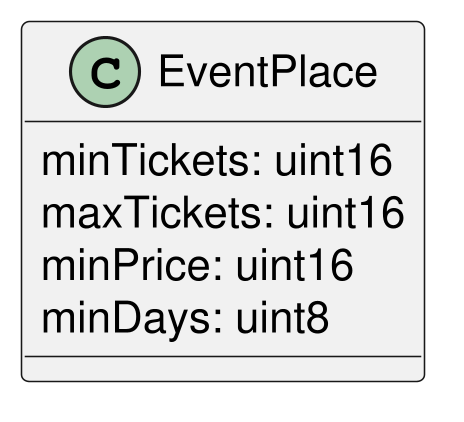
\includegraphics[width=0.95\textwidth]{./img/event-place.png}
\label{org11a36d1}
\end{center}

\begin{center}
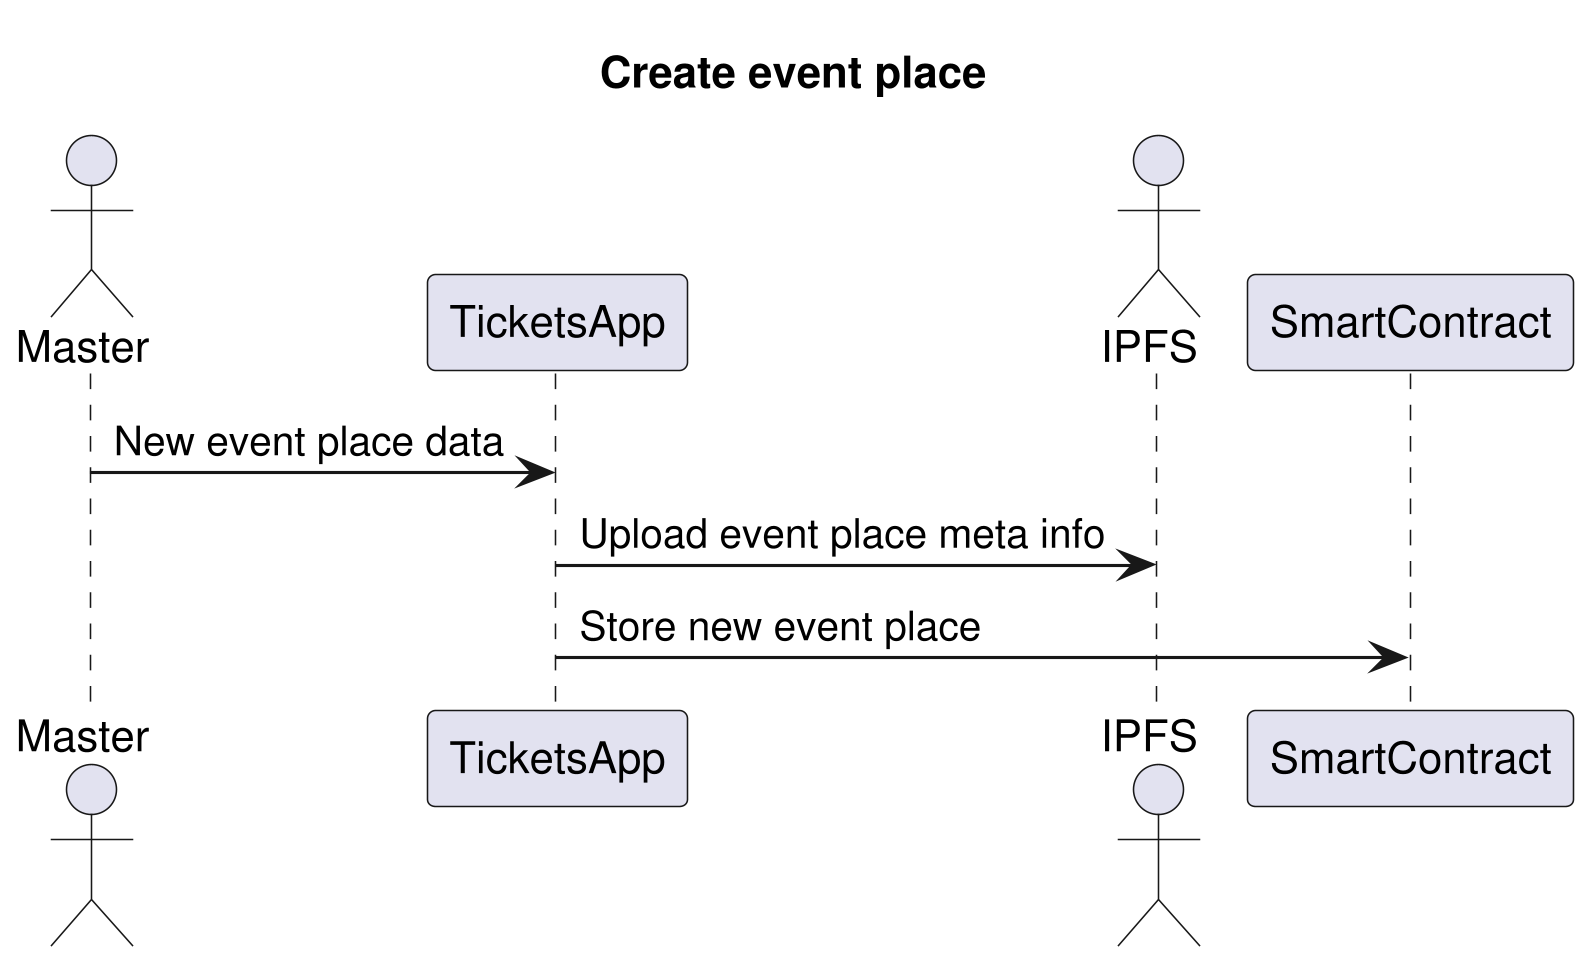
\includegraphics[width=0.95\textwidth]{./img/create-event-place.png}
\label{orgf6bef35}
\end{center}
\subsubsection{Save socials}
\label{sec:orgf9e0efd}

Supported socials:

\begin{itemize}
\item Telegram
\item Discord
\item Whats App
\item Instagram
\end{itemize}
\begin{enumerate}
\item V1
\label{sec:org35c2edf}

Used socials stored in the browser cache, so customer should input his social on each new device

\begin{center}
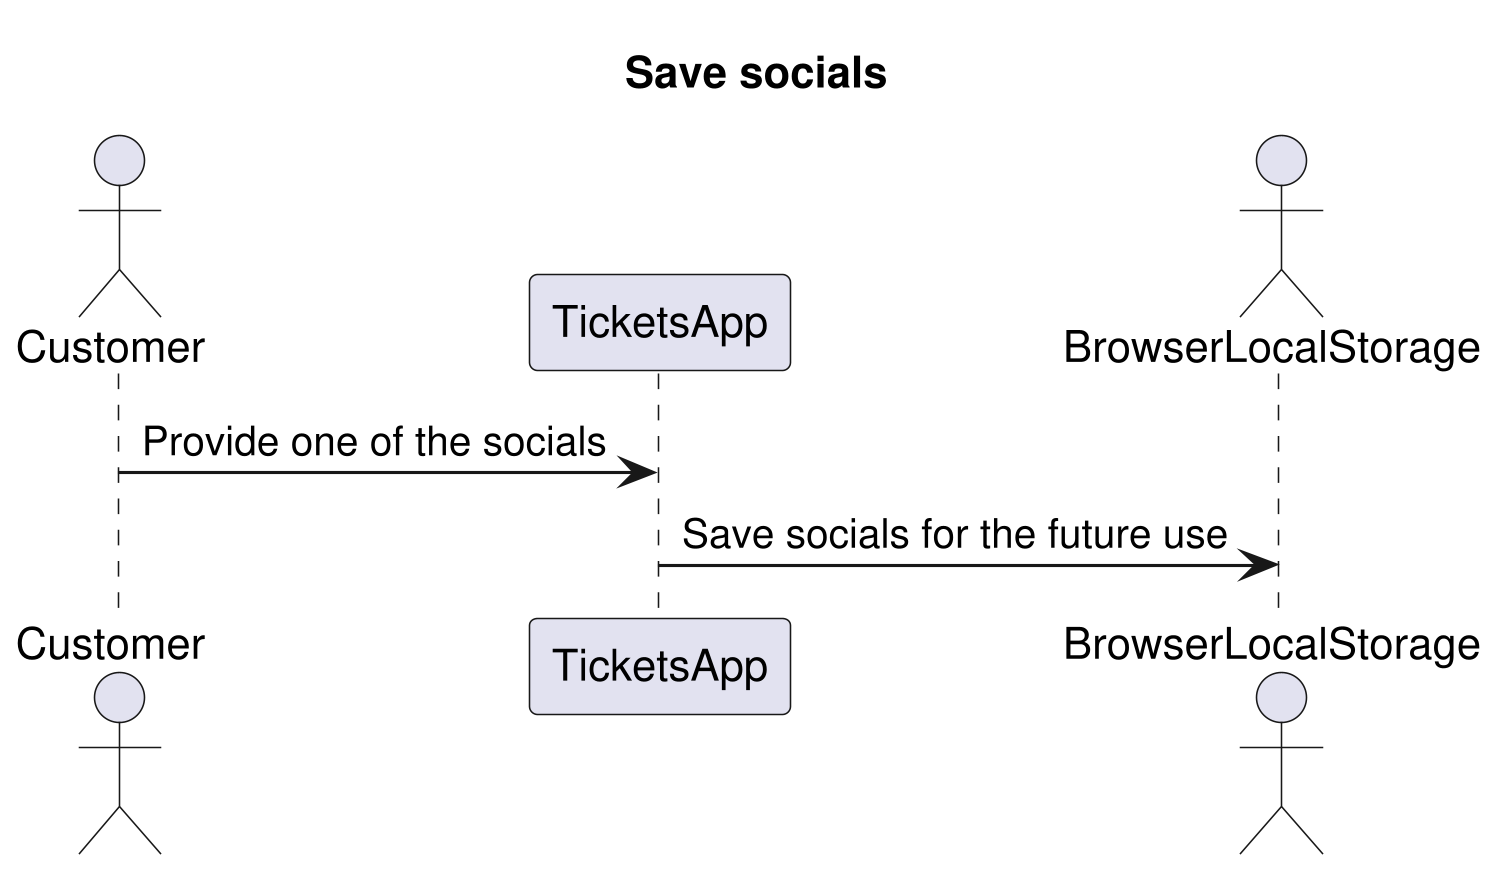
\includegraphics[width=0.95\textwidth]{./img/v1-save-socials.png}
\label{orge47d8e3}
\end{center}
\item V2
\label{sec:org9fe825c}

Used socials stored in the centralized database which allows to sync state of the all devices

\begin{center}
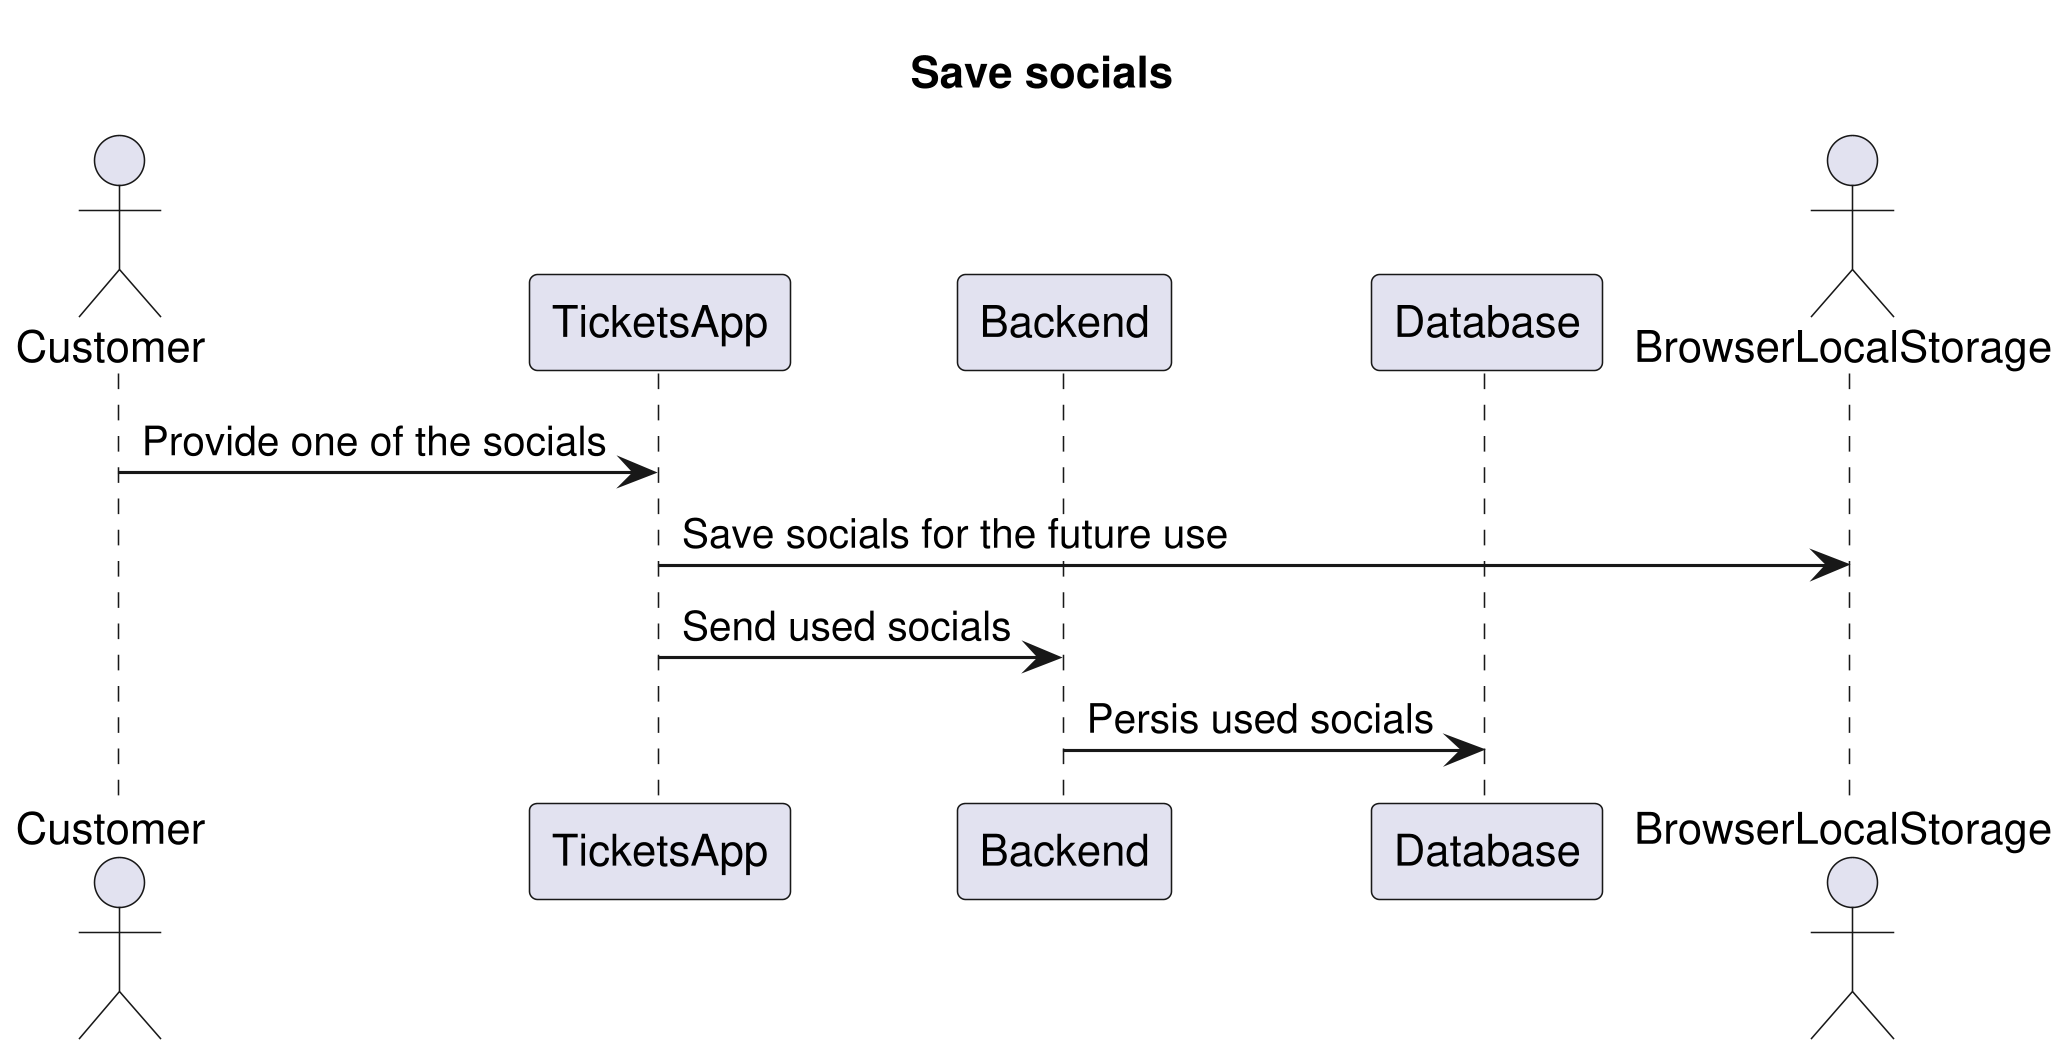
\includegraphics[width=0.95\textwidth]{./img/v2-save-socials.png}
\label{org7c6f8b3}
\end{center}
\end{enumerate}
\subsubsection{Submit event request}
\label{sec:org99ee9bc}

\begin{center}
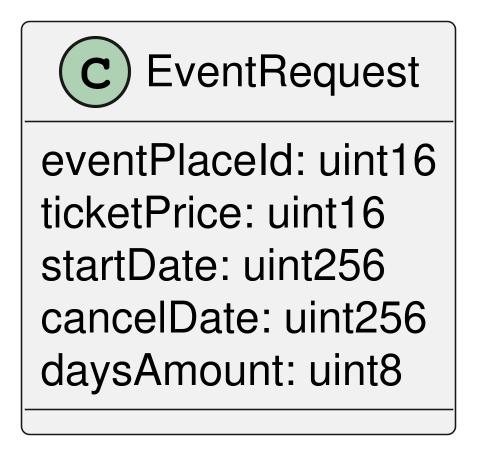
\includegraphics[width=0.95\textwidth]{./img/event-request.png}
\label{org9a64bfc}
\end{center}

\begin{center}
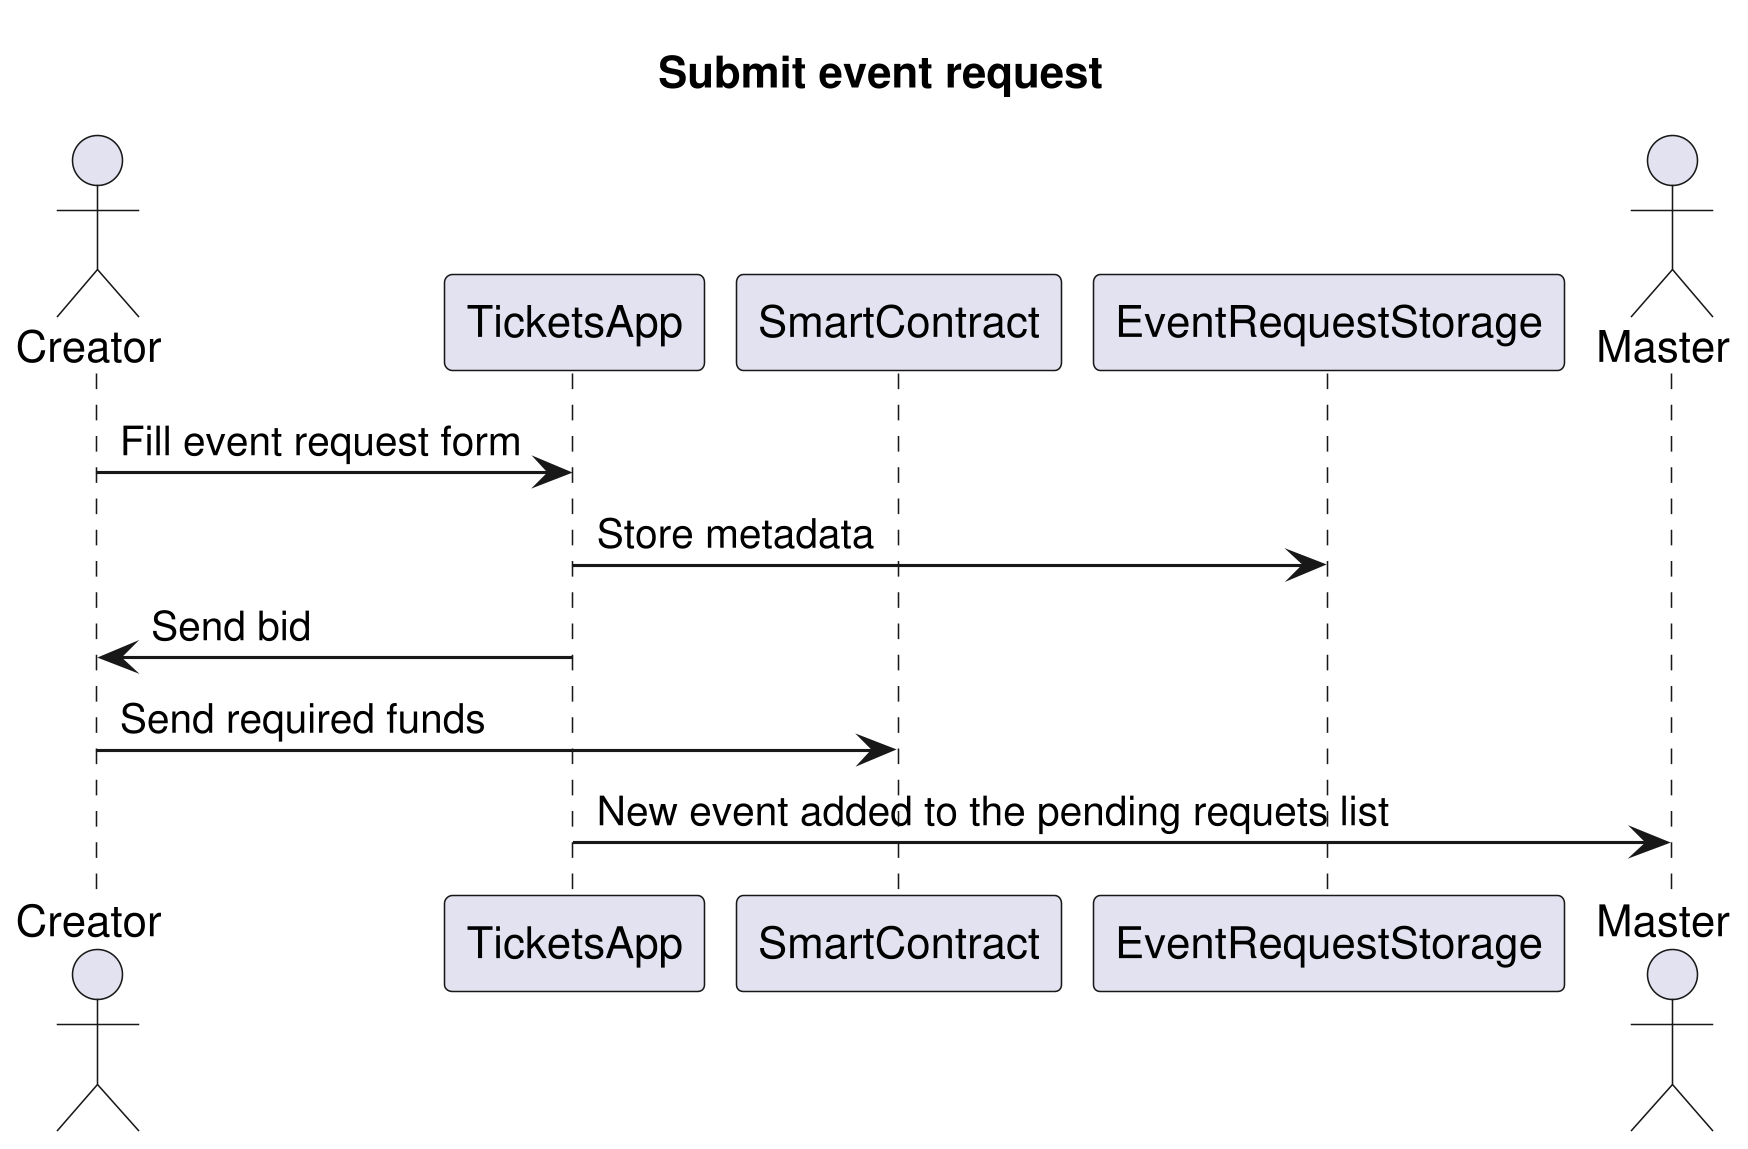
\includegraphics[width=0.95\textwidth]{./img/submit-event-request.png}
\label{org0238404}
\end{center}
\subsubsection{Approve event request}
\label{sec:org6dd85e9}

\begin{center}
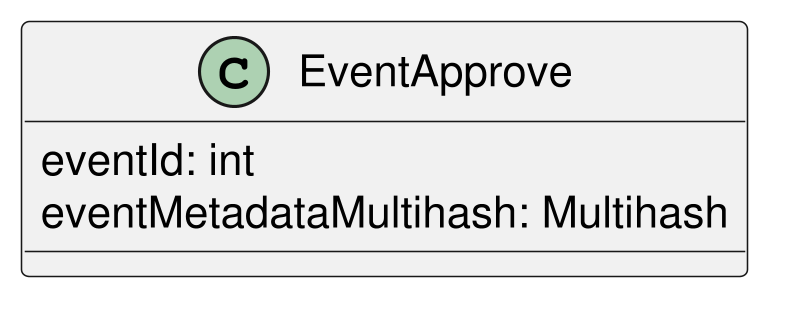
\includegraphics[width=0.95\textwidth]{./img/event-approve.png}
\label{org6d06529}
\end{center}

\begin{center}
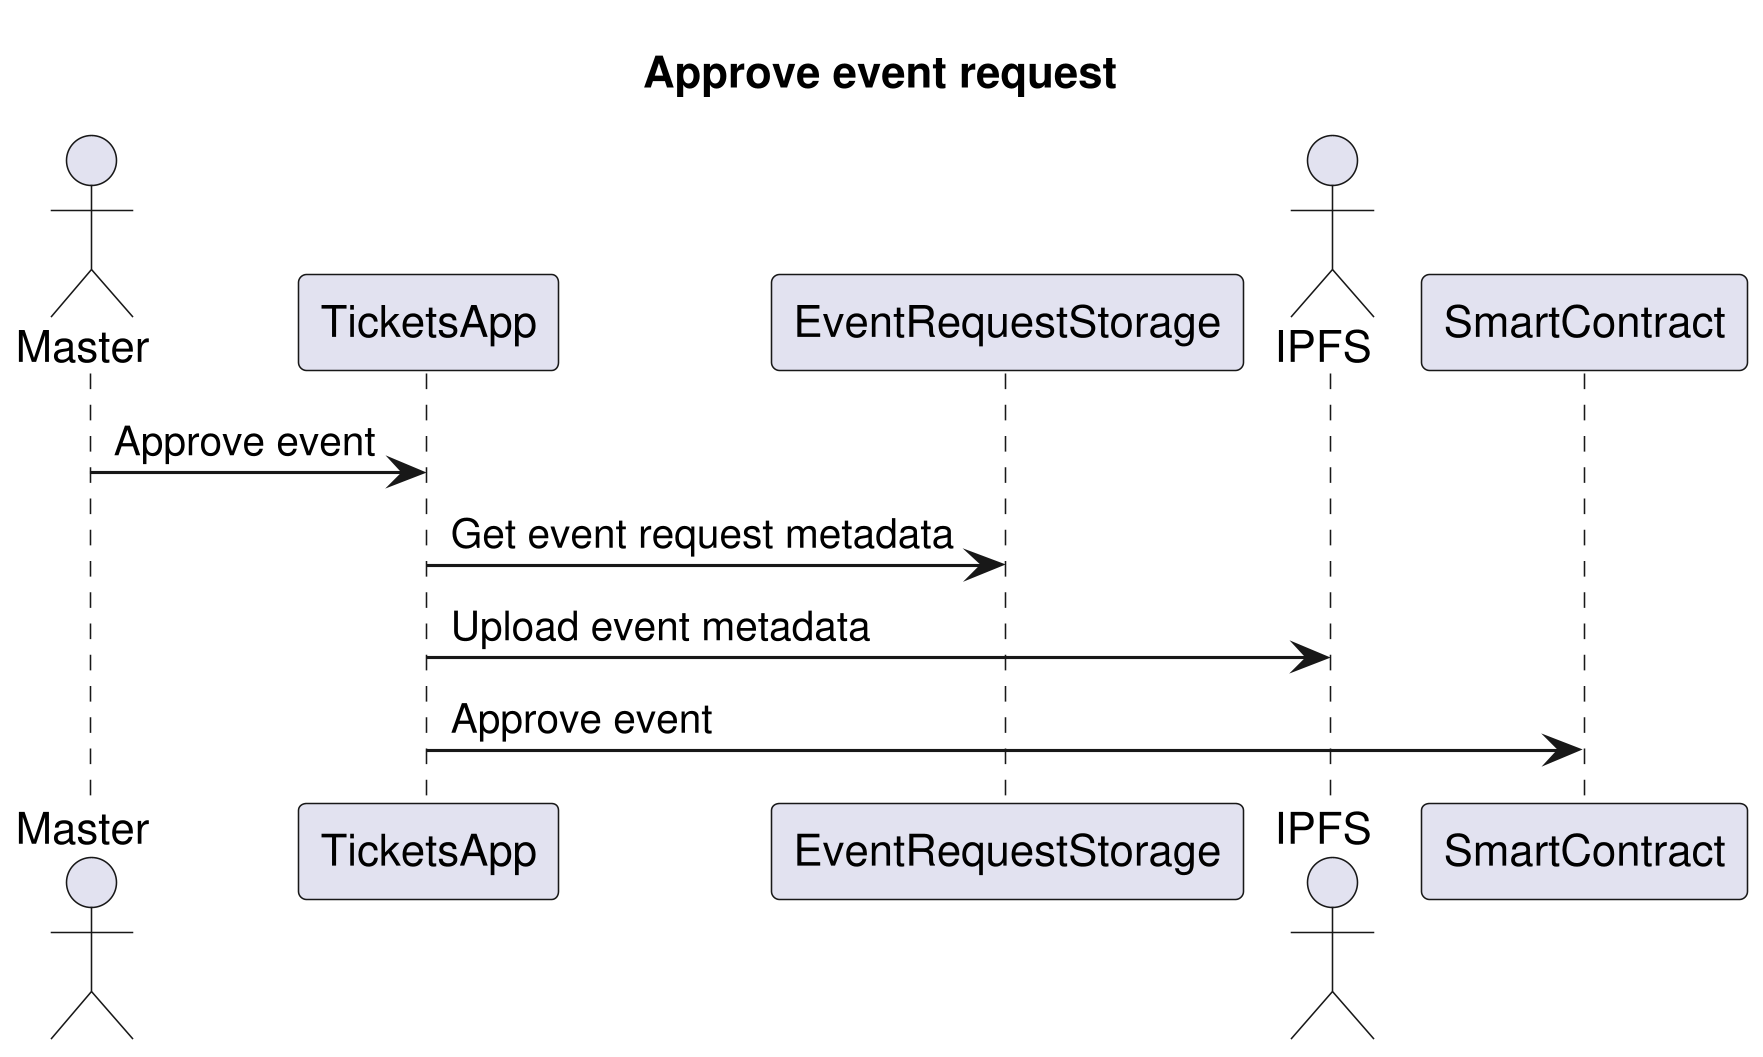
\includegraphics[width=0.95\textwidth]{./img/approve-event-request.png}
\label{org67cfabb}
\end{center}
\subsubsection{Edit event request}
\label{sec:orgd42e58c}

\begin{center}
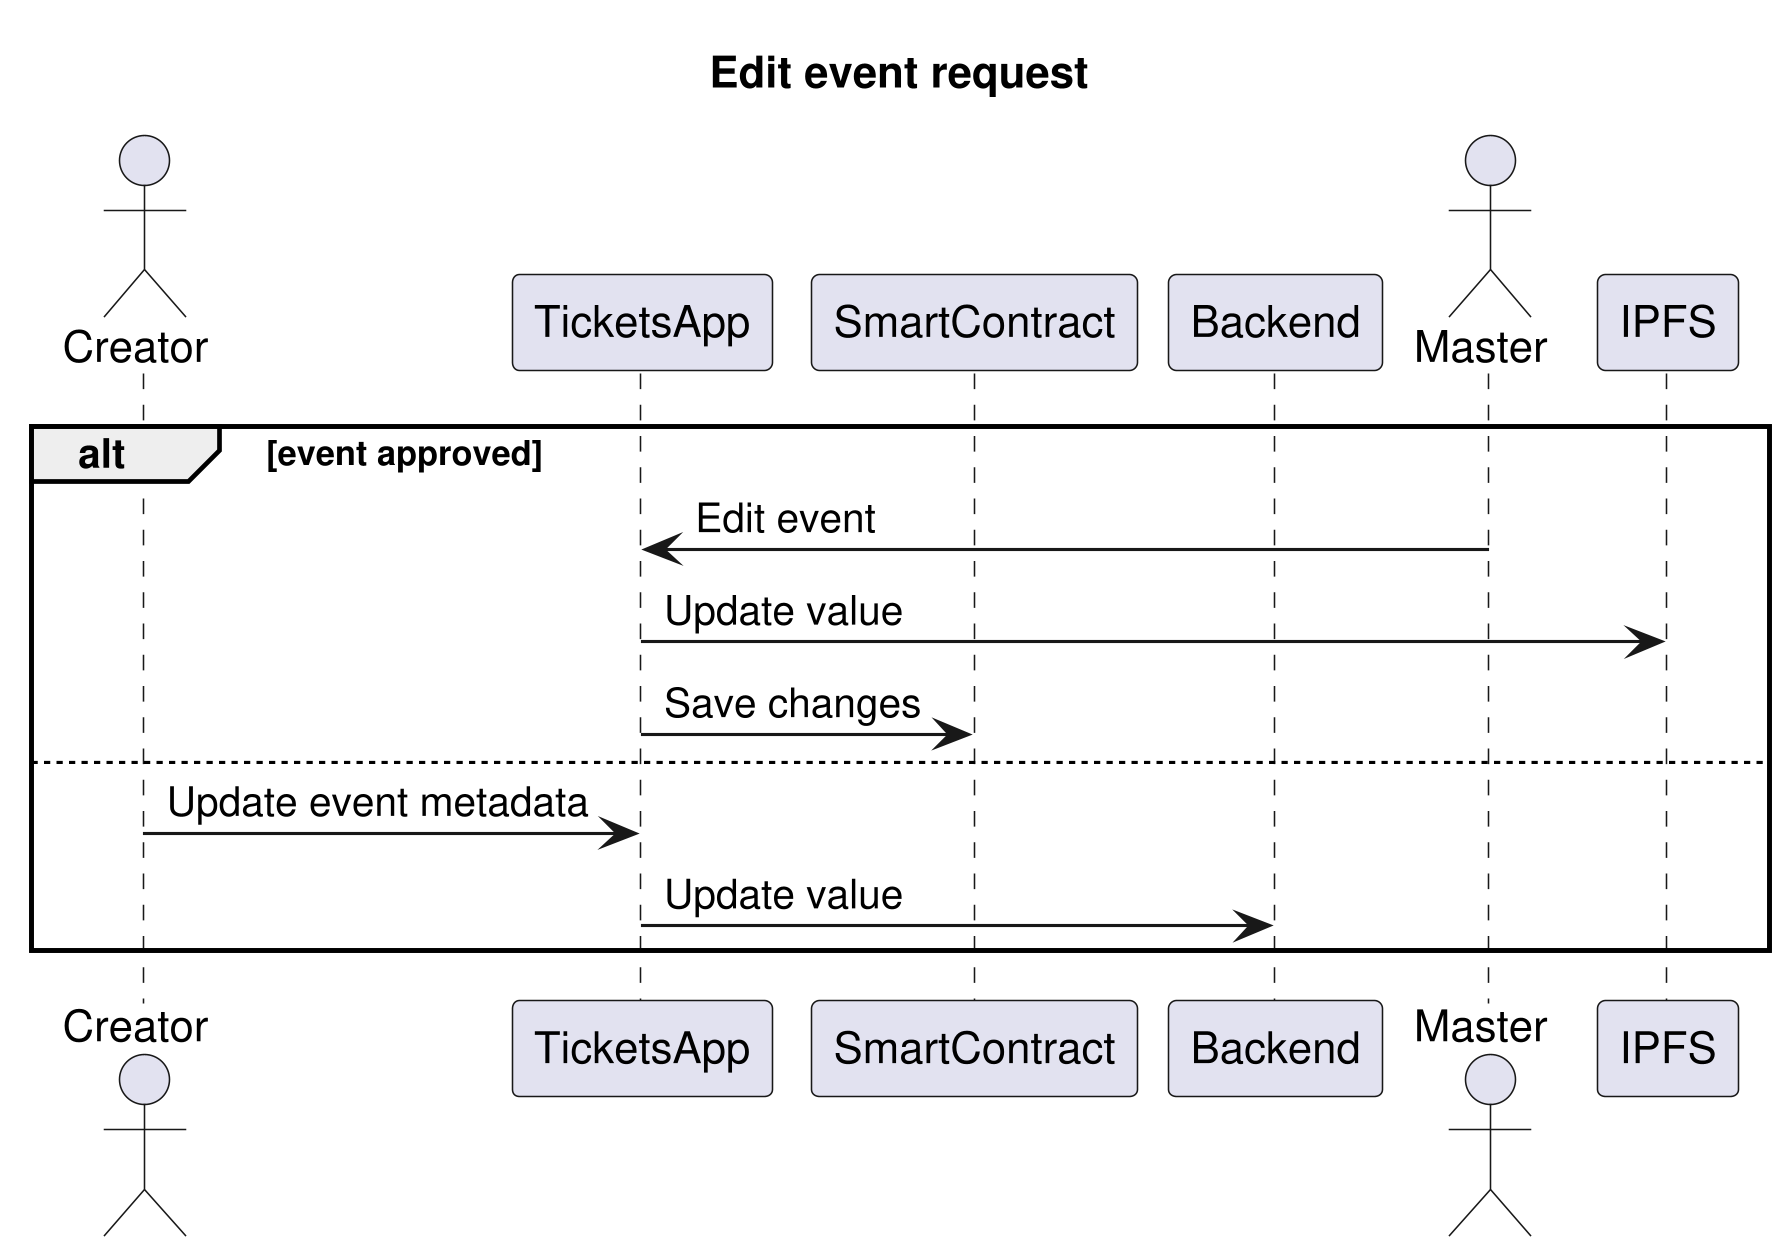
\includegraphics[width=0.95\textwidth]{./img/edit-event-request.png}
\label{org3f988f8}
\end{center}
\subsubsection{List events}
\label{sec:org3fb6b97}

\begin{center}
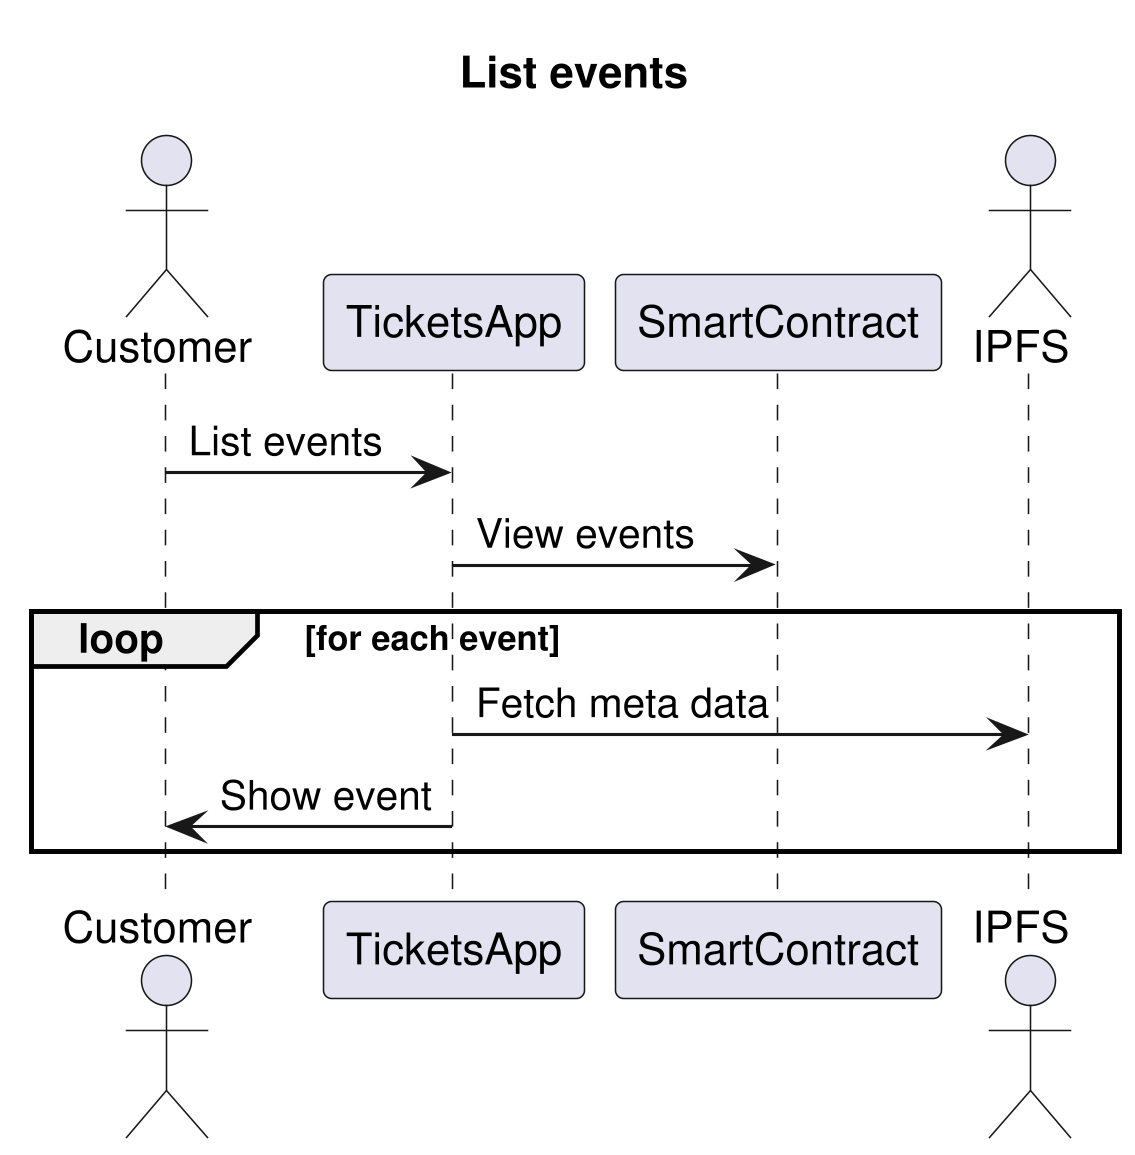
\includegraphics[width=0.95\textwidth]{./img/list-events.png}
\label{orgc038a26}
\end{center}
\subsubsection{Buy ticket}
\label{sec:org9777165}

\begin{enumerate}
\item V1
\label{sec:orgfb97a09}
\begin{center}
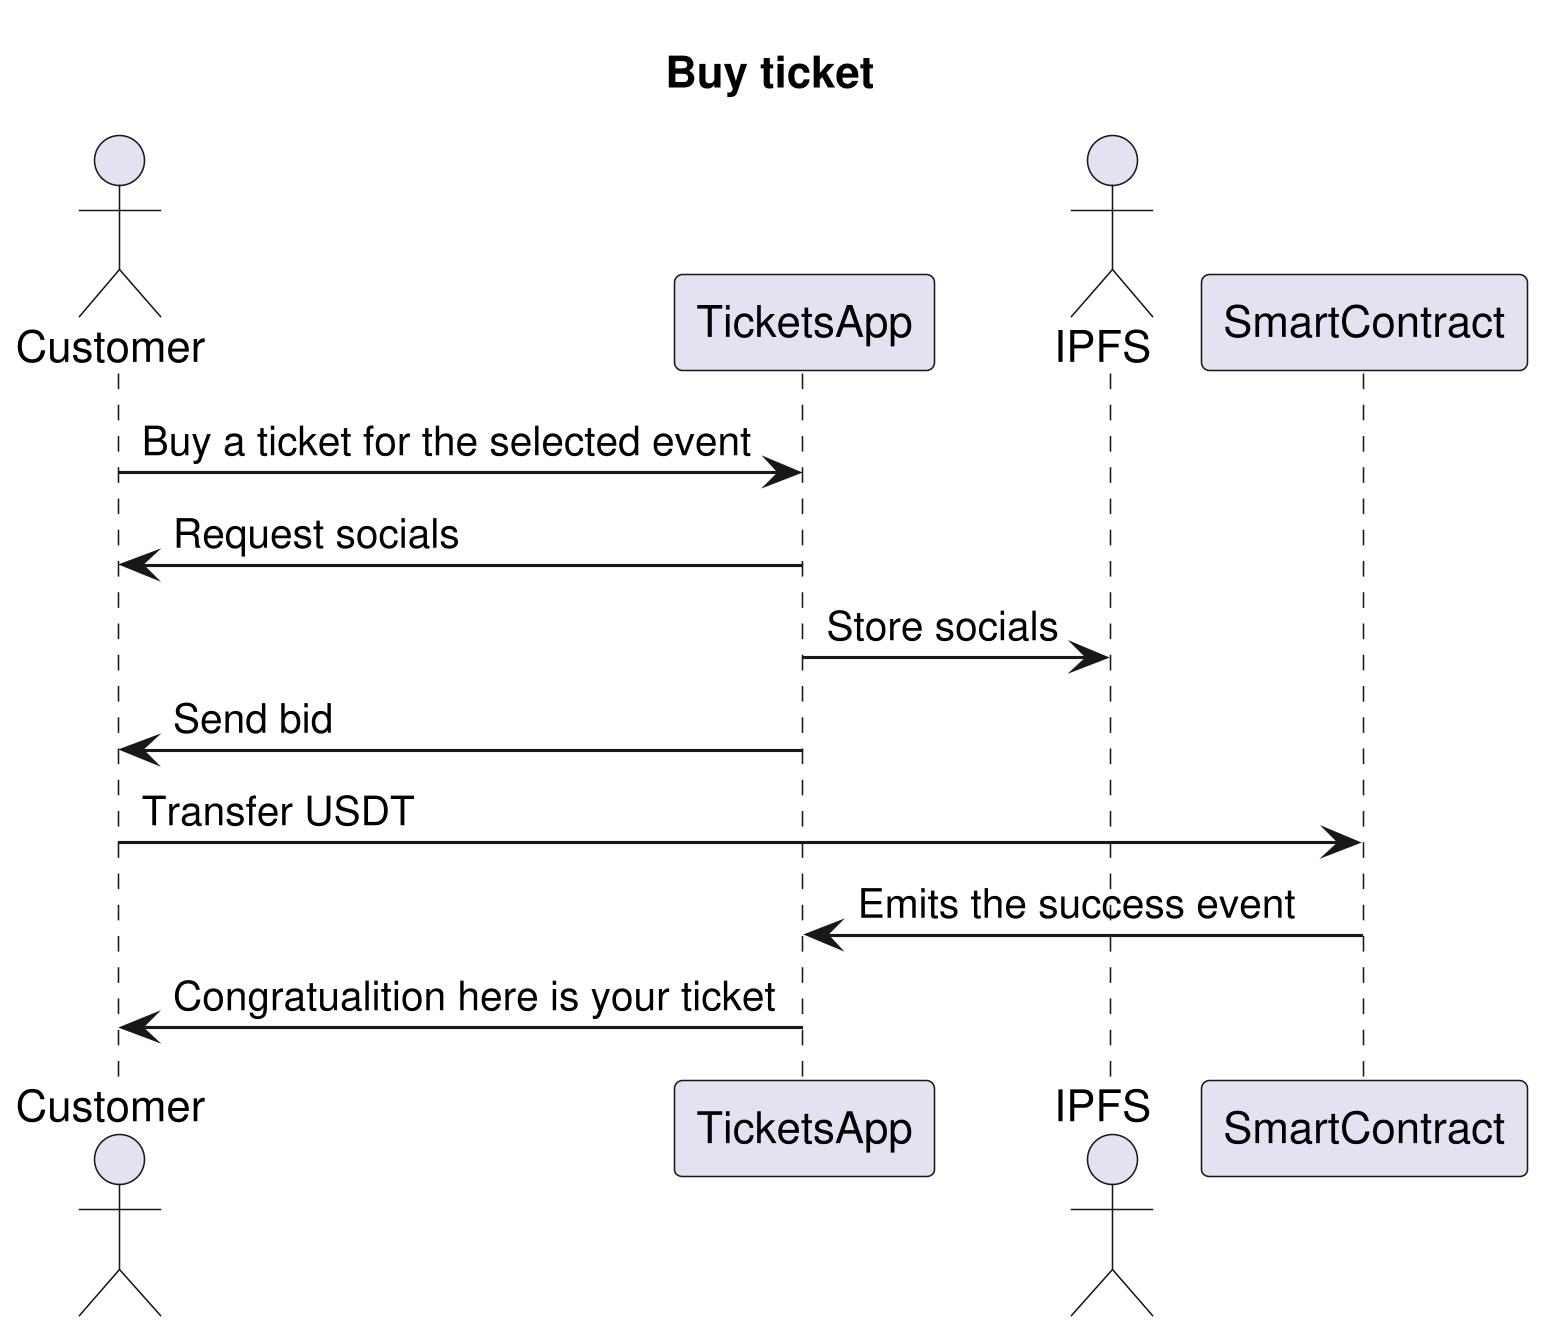
\includegraphics[width=0.95\textwidth]{./img/v1-buy-ticket.png}
\label{orgc790f98}
\end{center}
\item V2
\label{sec:org04cca44}
\begin{center}
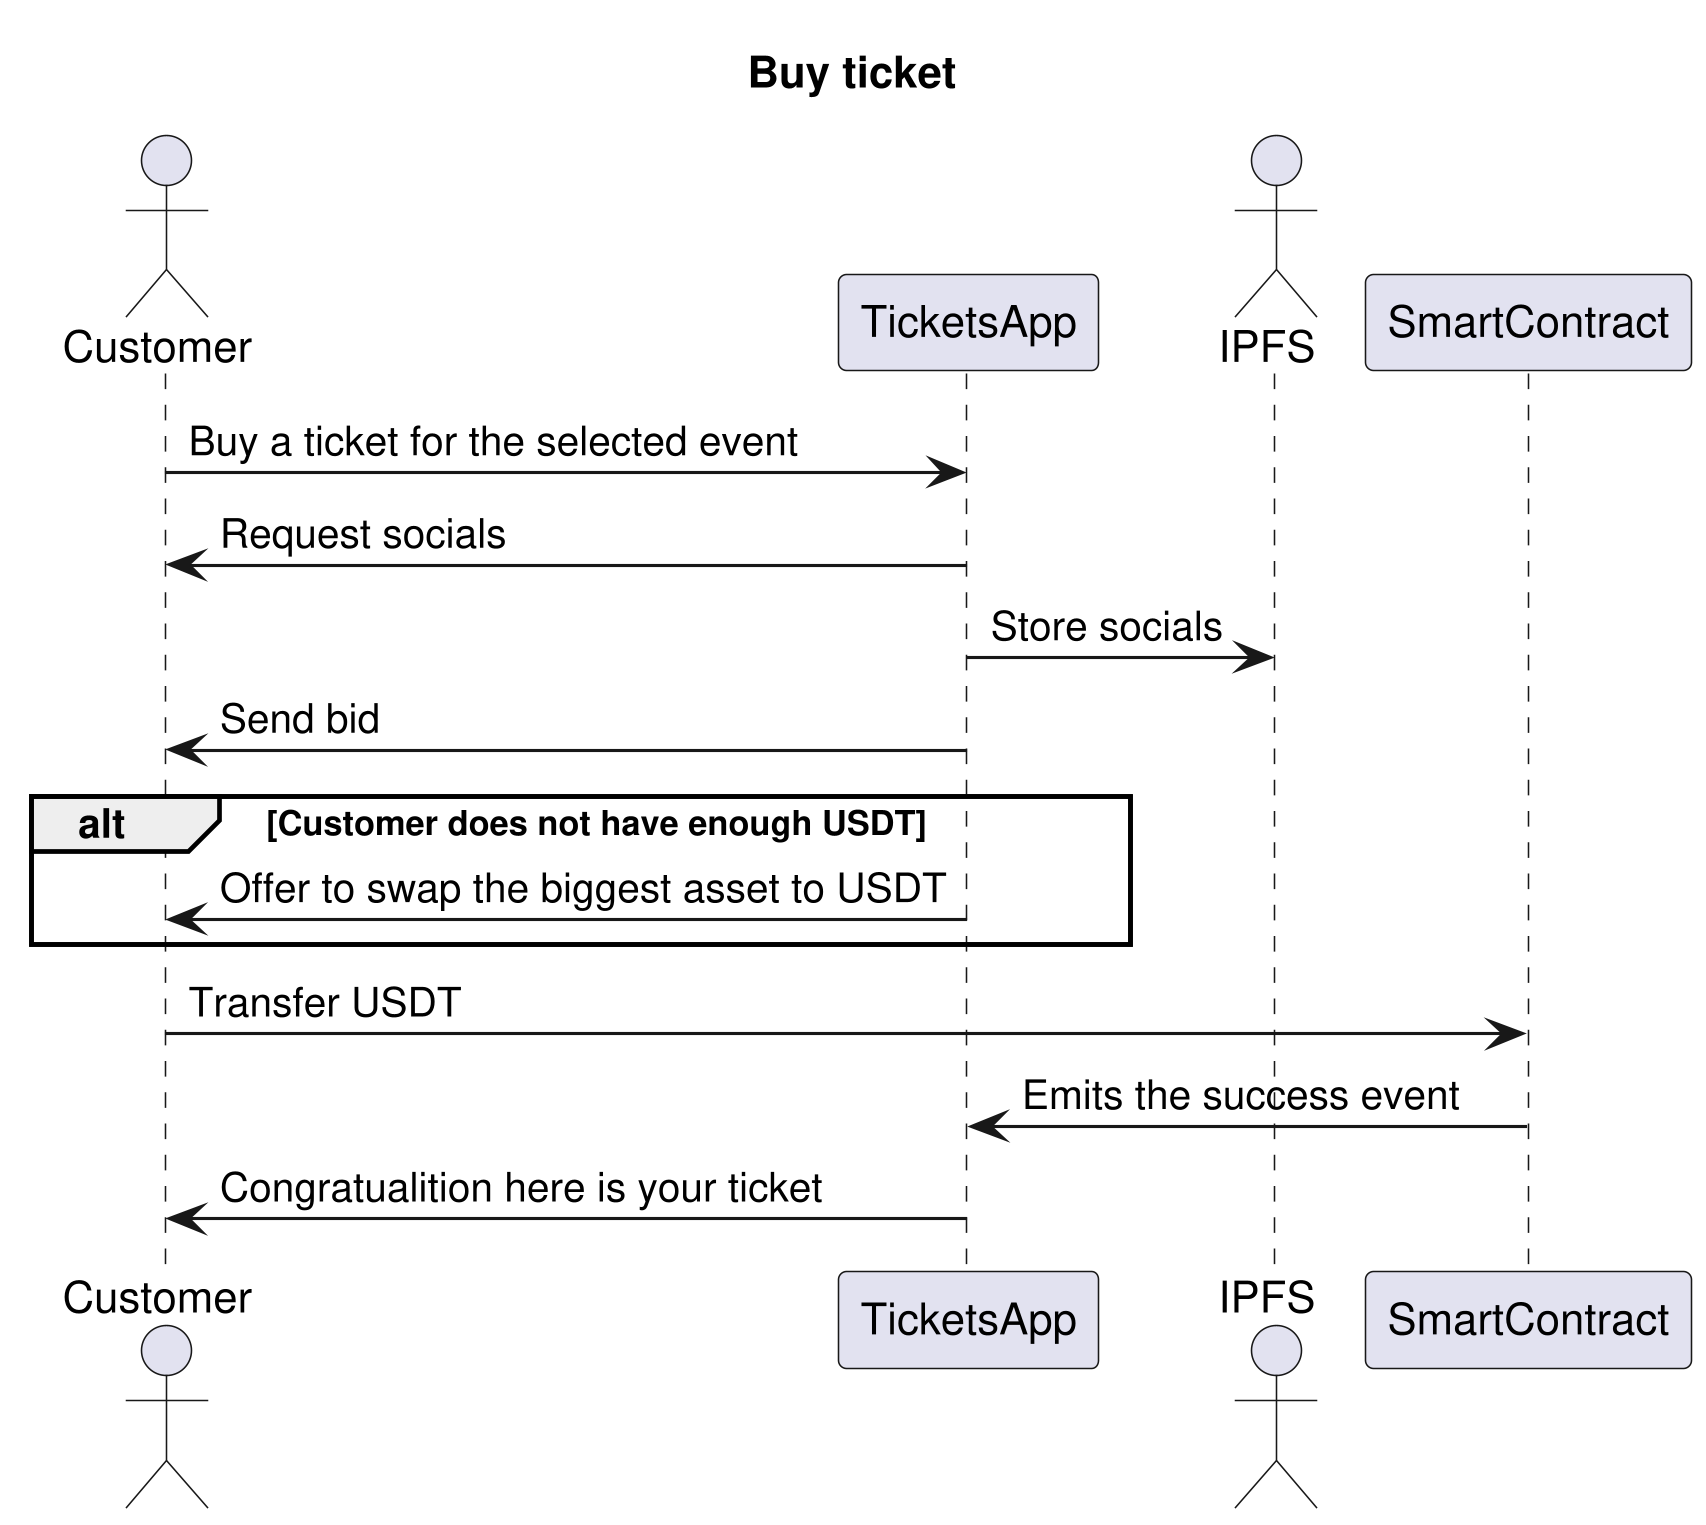
\includegraphics[width=0.95\textwidth]{./img/v2-buy-ticket.png}
\label{org055ca5d}
\end{center}
\end{enumerate}
\subsubsection{Assign event's staff}
\label{sec:org577bacb}

This could be changed to the array of staff independent from the event which can be edited by the master.

Also given approach makes it difficult to list events for the given staff's address and requires GAS for each edit.

As and alternative we can store staff addresses in the IPFS, but it'll introduce some latency in exchange of less GAS cost.

\begin{center}
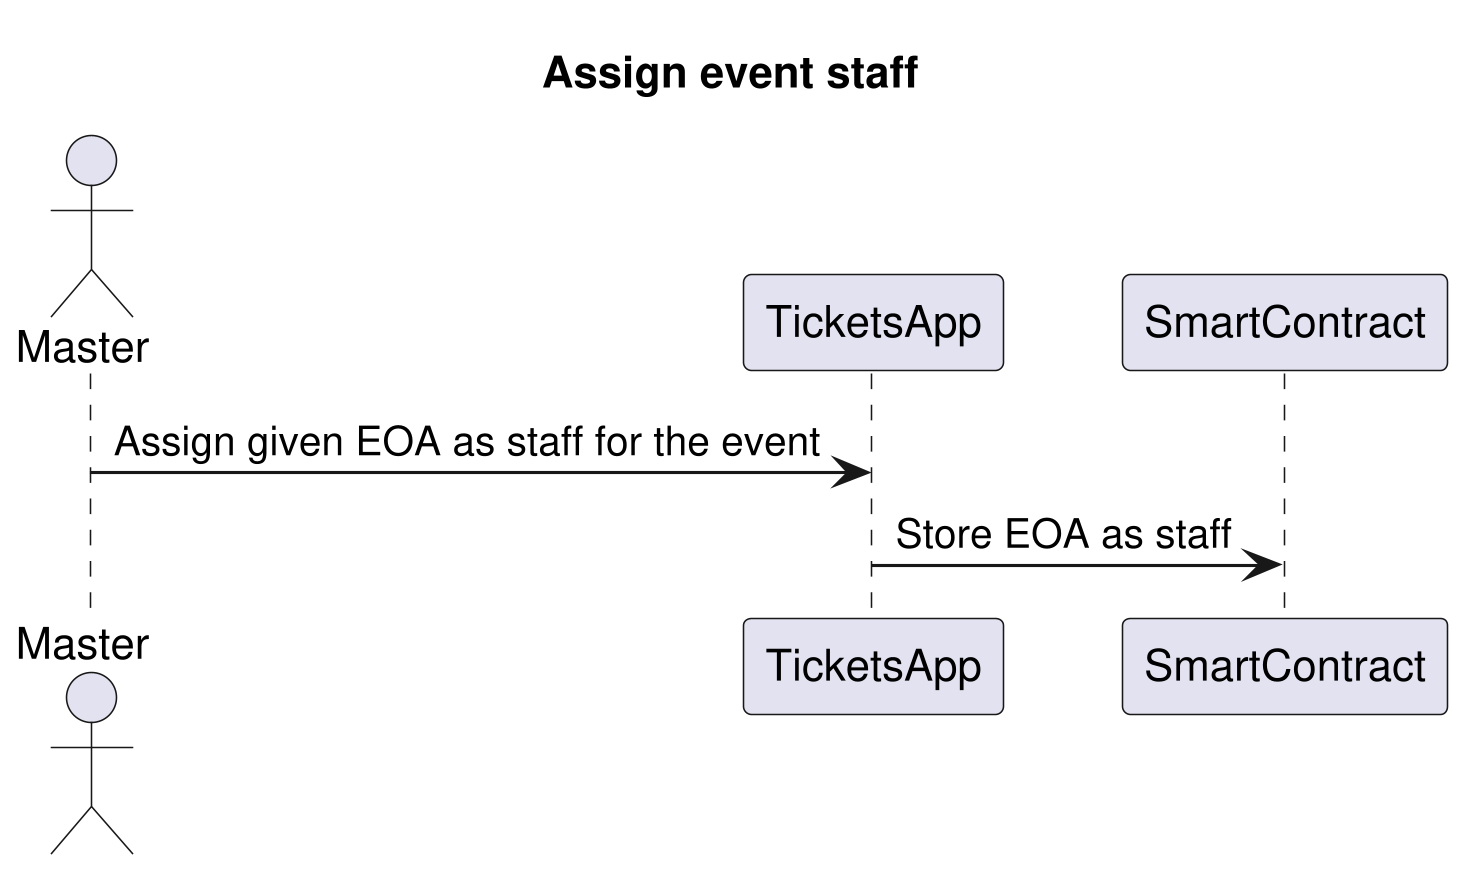
\includegraphics[width=0.95\textwidth]{./img/assign-event-staff.png}
\label{org8e9f852}
\end{center}
\subsubsection{Show ticket}
\label{sec:orgaccd666}

\begin{center}
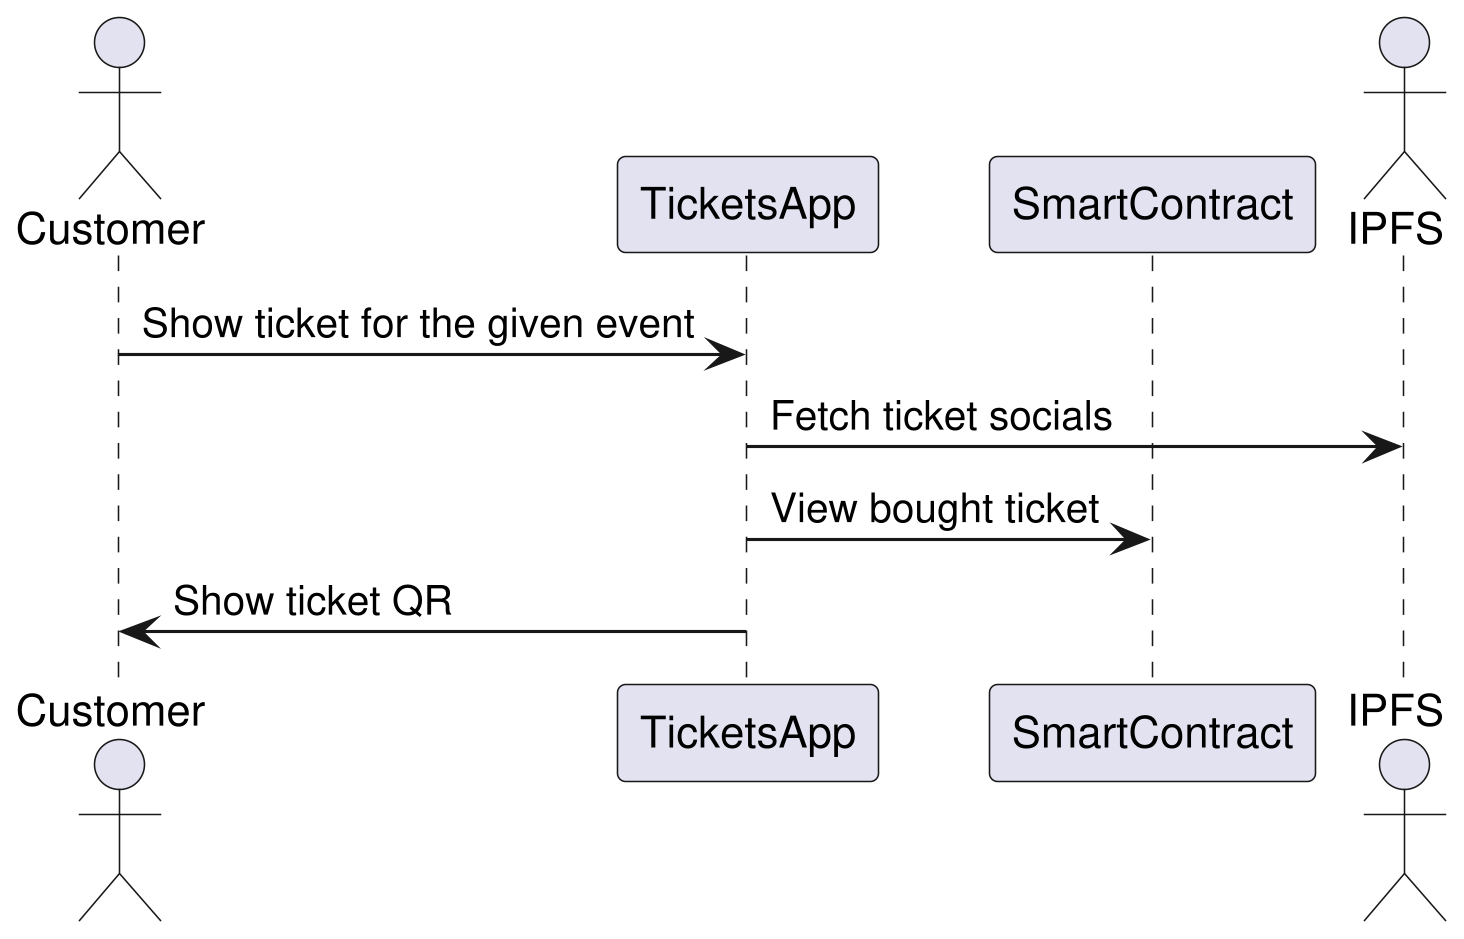
\includegraphics[width=0.95\textwidth]{./img/show-ticket.png}
\label{orgcd8b5d5}
\end{center}
\subsubsection{Verify bought ticket}
\label{sec:orgd59a908}

\begin{center}
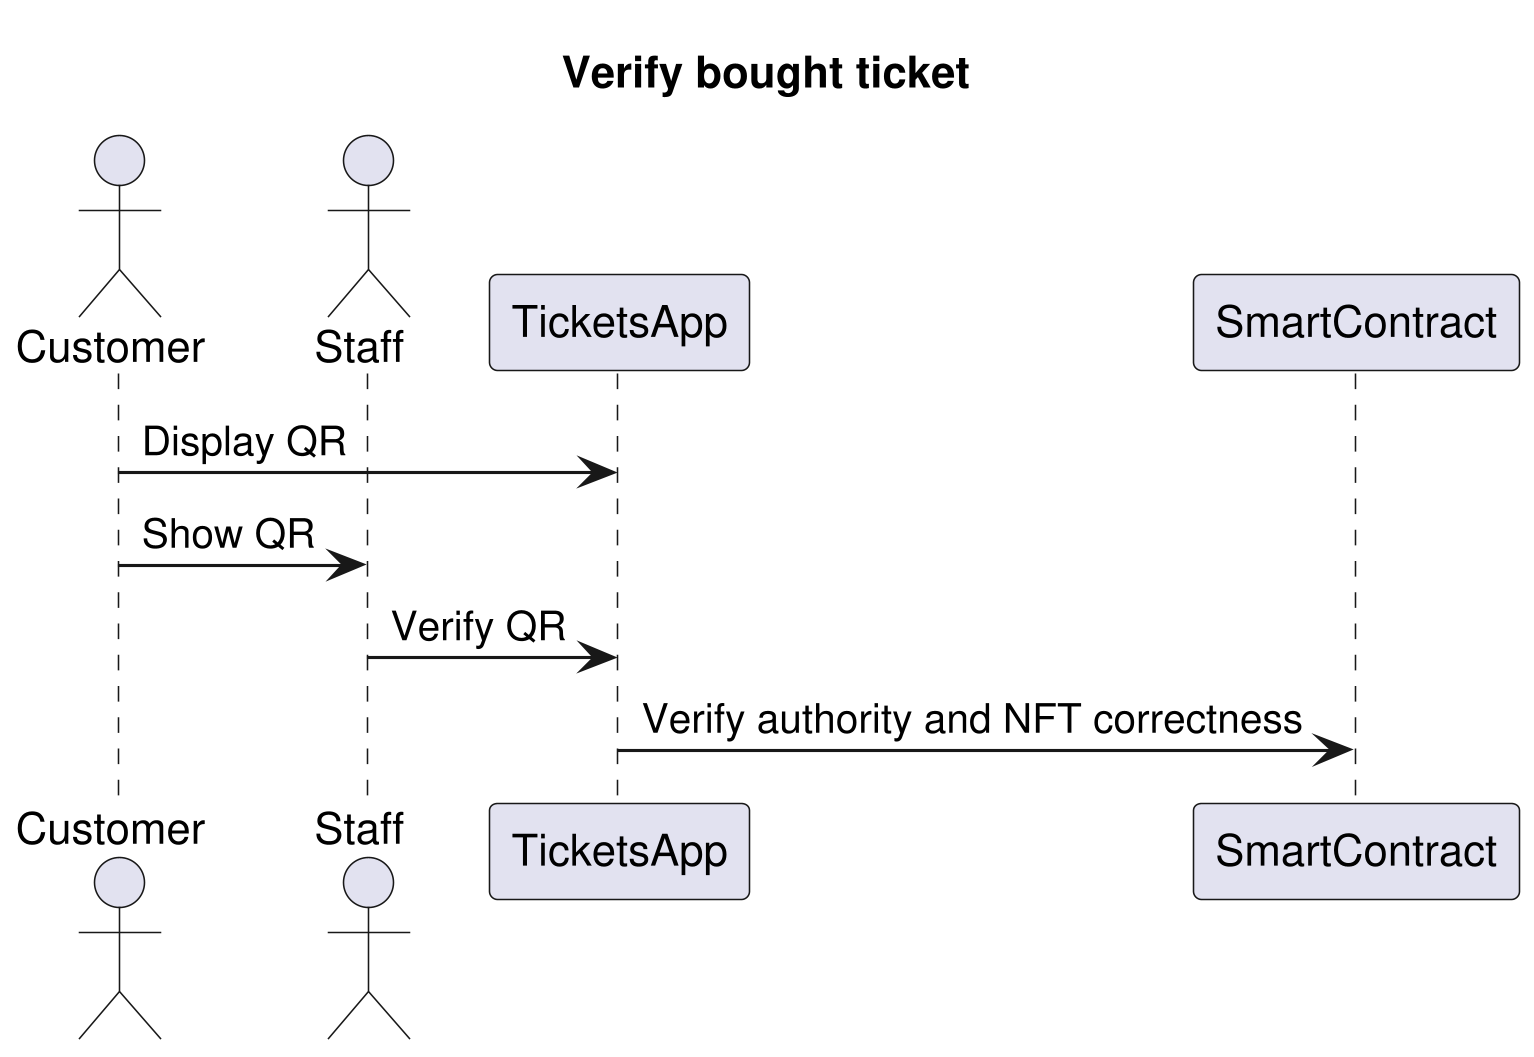
\includegraphics[width=0.95\textwidth]{./img/verify-bought-ticket.png}
\label{org9982c1b}
\end{center}
\subsubsection{Cancel Event}
\label{sec:org668879d}

\begin{center}
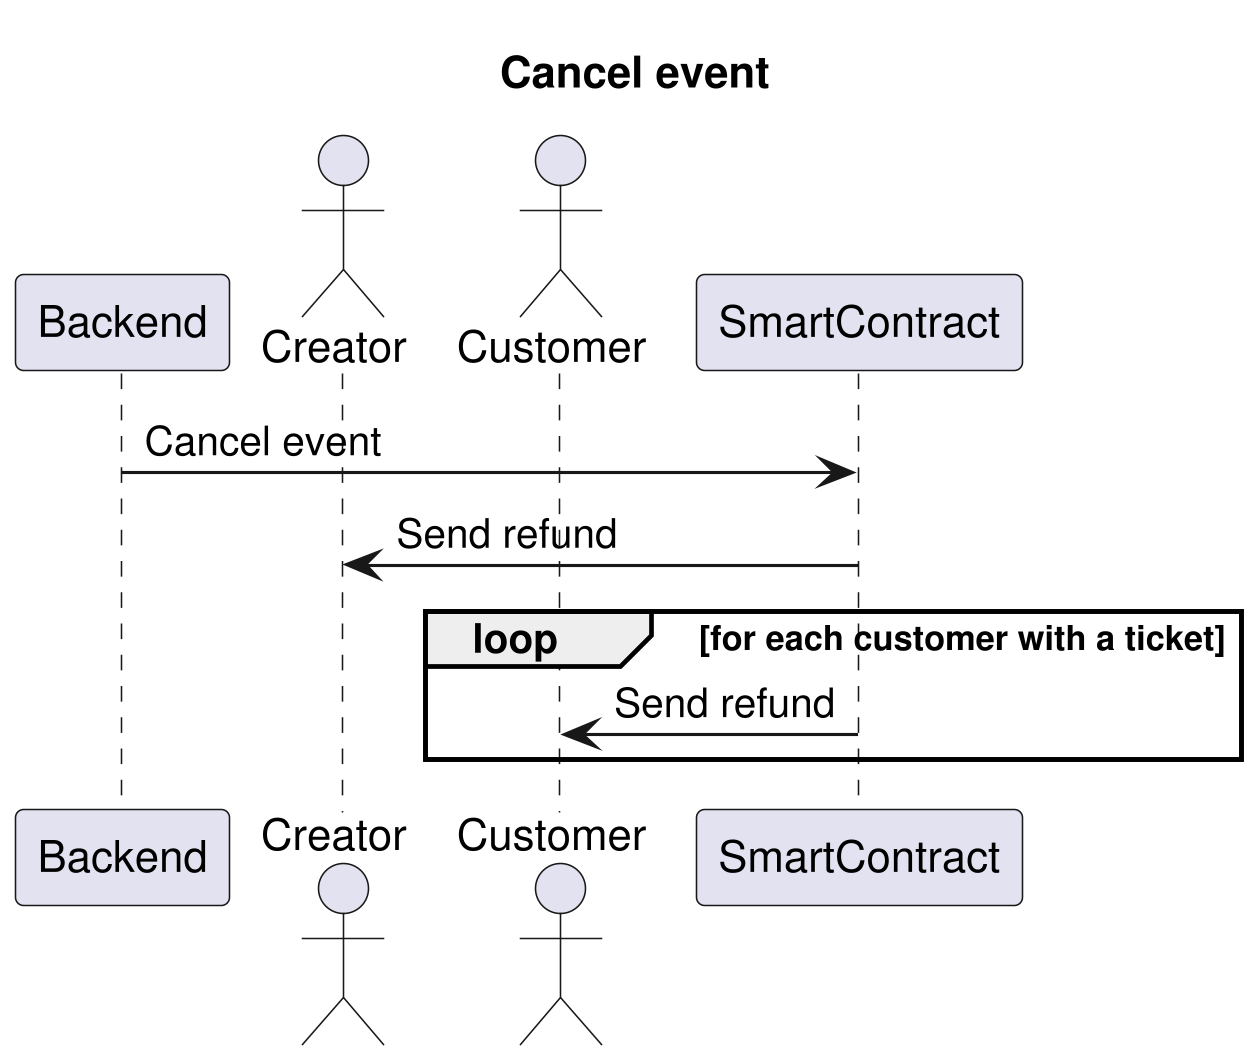
\includegraphics[width=0.95\textwidth]{./img/cancel-event.png}
\label{org67893fe}
\end{center}
\subsubsection{Close event}
\label{sec:orgcbeb0a1}

\begin{center}
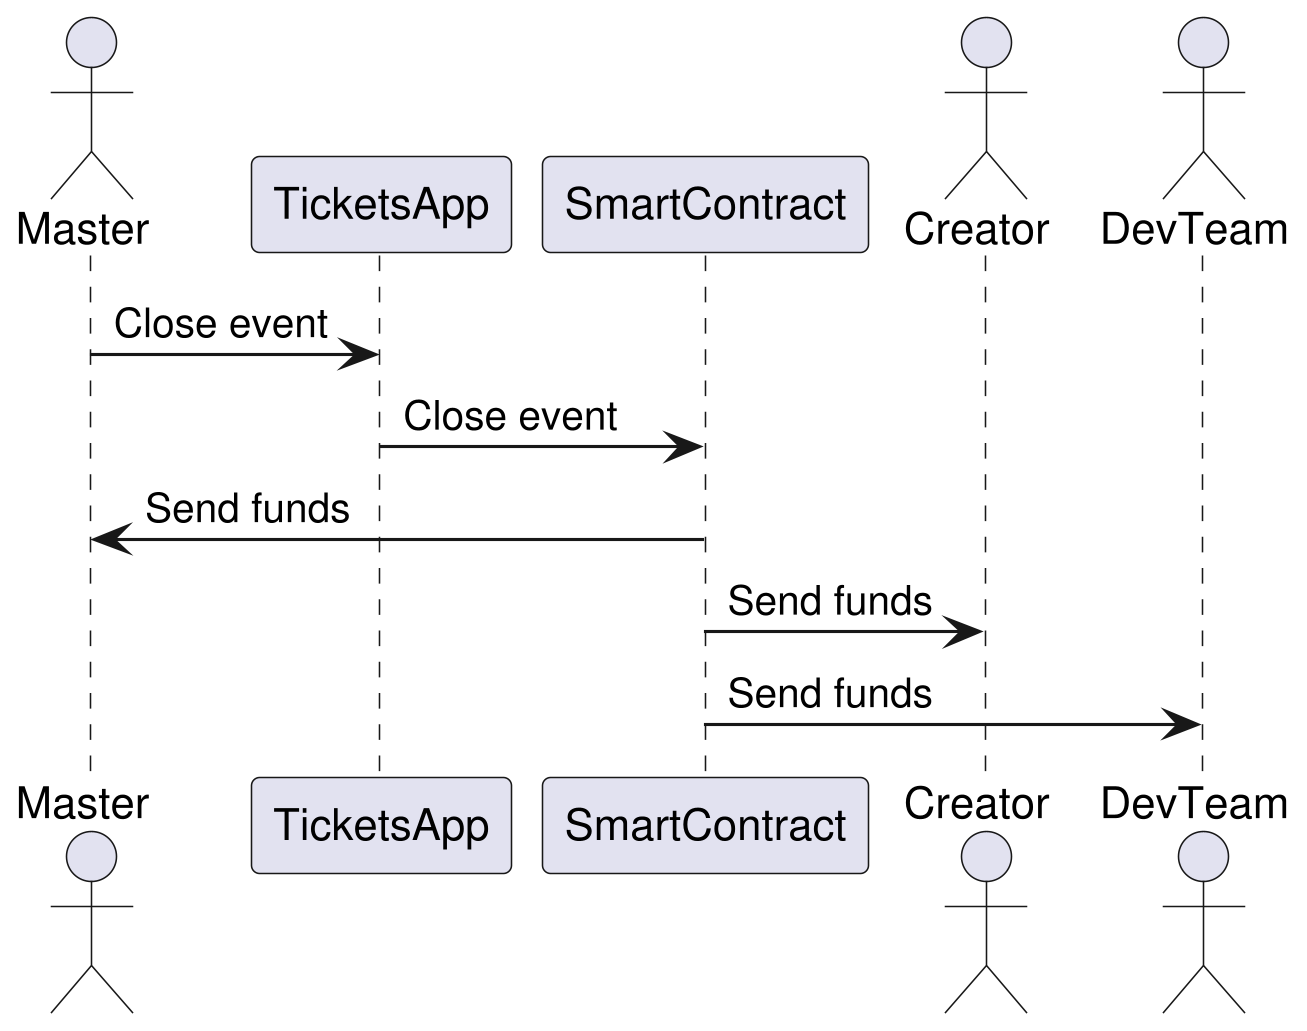
\includegraphics[width=0.95\textwidth]{./img/close-event.png}
\label{orgbb09c29}
\end{center}
\subsection{Tech stack}
\label{sec:org81f95ae}

Solidity, OpenZeppelin, React, TypeScript, Tailwind, ethers.js, IPFS

Also a thin backend over database is required to provide free of charge ability to change event request data before it's approve, so it'll be implemented with Python, SQLite and Litestar
\subsection{Excluded features from the first stage}
\label{sec:orgd0c60c9}

Given list of features can be interpreted as obviously required or any section below can unintentionally imply them, so they explicitly mentioned

\begin{itemize}
\item Tickets refund
\item Cancel or refund event request submission
\item Any sort of push notifications about any updates or new data
\item Ticket price change on sold out and increasing available seats
\item Remove assigned staff person to the event
\end{itemize}
\subsection{Proxy contract vs multiple versions}
\label{sec:org36915b4}

Because of big amount of reads from the blockchain (which lead to spending gas on call delegation in proxy) we offer to use multiple versions and support them on the client side. To prevent difficulties of funds \& data migration between versions, we'll create new events in a new version, but still support the previous ones until all events there will be closed or canceled.
\section{Questions}
\label{sec:org047244f}

\subsection{Both desktop and mobile are required?}
\label{sec:org72f3a1a}

\begin{quote}
Mobile only
\end{quote}
\subsection{Is it required to verify tickets without internet connection?}
\label{sec:org835bd6b}

\begin{quote}
No
\end{quote}
\subsection{Will be there multiple masters or the only one in foreseeable future?}
\label{sec:org75abab5}

\begin{quote}
Only one
\end{quote}
\subsection{Event request price fixed in ETH, depends on ETH/USD rate or could be changed by the master?}
\label{sec:org17ca663}

\begin{quote}
Smart contract should work with USDT
\end{quote}
\subsection{Is a ticket transfer allowed e.g. customer A bought a ticket, but sent it to the customer B?}
\label{sec:org61553ee}

\begin{quote}
Yes
\end{quote}

It requires additional UI and flows to properly update ticket's meta data, so this feature will be skipped in the V1
\subsection{Will tickets have some metainfo about the owner (name, number etc)}
\label{sec:org1f5e285}

\begin{quote}
Yes, socials i.e. one or many \{Telegram, Discord, Instagram, Whats App\}
\end{quote}
\subsection{Is it applicable to show available seats count for all (so the creator and master can see it as well without additional screen)?}
\label{sec:orge87d6b0}

\begin{quote}
Yes
\end{quote}
\subsection{UI design references}
\label{sec:org0d78ade}
\end{document}
